% !TeX root = main.tex

\chapter{Real time reccurent learning}

A partir de cette section, les objectifs sont de reconnaitre une chaine de caractère en temps réel. C'est à dire que en donnant un ou plusieurs caractères, on doit être capable de prédire la fin de la chaine. Ce genre de problème peut être étendu à la recherche comportementale en temps réel. Pour résoudre ce genre de problème, on utilise des réseaux neuronaux récurrents, qui ont l'avantage de se souvenir des états précedents pour pouvoir prédire efficacement les états suivants. Dans un premier temps, nous allons nous interesser aux réseaux RTRL.

\section{Théorie}

Dans la suite, nous allons nous interesser au problème de la grammaire de Reber, qui servira d'échantillon test pour RTRL.

\subsection{La grammaire de Reber}

 Une grammaire de Reber est un langage défini par l'automate déterministe cyclique suivant :
 
\begin{figure}[!ht]
\begin{center}
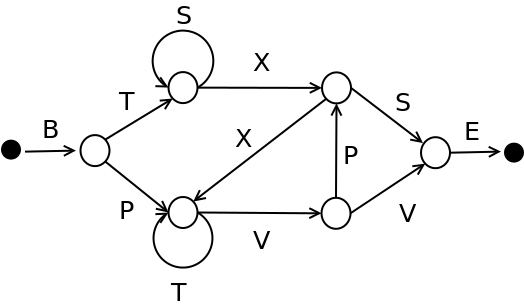
\includegraphics[height=5cm]{rtrl/reberGrammar.png}
\end{center}
\caption{Grammaire de Reber simple}
\end{figure}

 
De base, on considère une probabilité uniforme de chosir l'état suivant parmis les états possibles suivants. La lettre $B$ et la lettre $E$ sont des lettres indiquant simplement le début et la fin du perceptron, elle n'ont pas d'interet propre pour la grammaire. Les autres lettres présentes sur les arètes peuvent variés, mais elles doivent respecter les règles suivantes :
\medskip
\begin{itemize}
	\item Chaque lettre doit apparaitre exactement deux fois
	\item On ne peut pas obtenir deux lettres consécutives en passant par des états différents.
\end{itemize}

\vspace{\parskip}
L'interet de la grammaire de Reber est que c'est un automate simple qui ne nécessite que la mémoire de la dernière et de l'avant dernière lettre pour trouver la suivante. En effet, d'après la dernière règle, connaitre les deux dernières lettres impose l'état actuel dans l'automate. En outre, chaque lettre apparaissant deux fois, la connaissance seule de la dernière lettre ne suffit pas à prédir la suivante correctement. On remarque que l'on peut résoudre ce problème avec un perceptron classique si on donne en entrée du perceptron les deux dernières lettres du mot.